\begin{figure}[!ht]
    \centering
        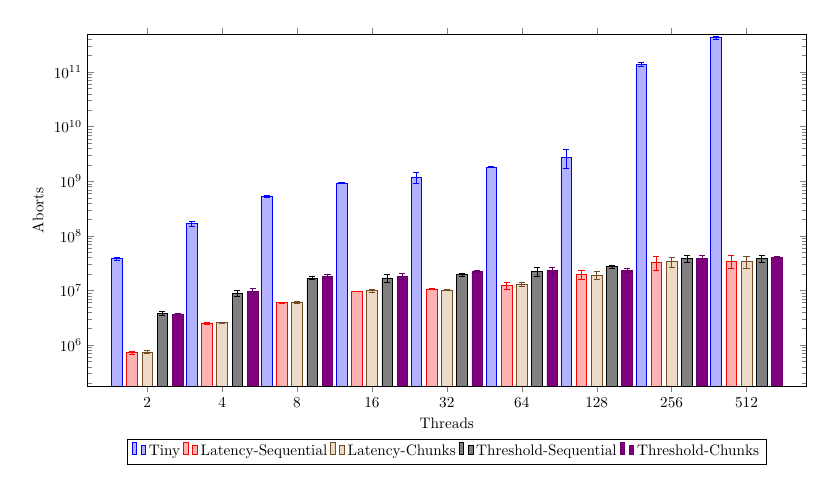
\begin{tikzpicture}[scale=0.55, baseline]
        \begin{axis}[
            ymode=log,
            width=1.5 \linewidth,
            height=0.8 \linewidth,
            %media de tempo intruder
            ybar=3pt,
            %enlargelimits=0.10,
            legend style={at={(0.5,-0.15)}, anchor=north, legend columns=-1},
            ylabel=Aborts,
            xlabel=Threads,
            symbolic x coords={1, 2, 4, 8, 16, 32, 64, 128, 256, 512},
            xtick=data,
            ymin=0,
            ymax=490000000000,
            bar width=7pt,
            % nodes near coords,
            nodes near coords align={vertical},
        ]
        \addplot+[error bars,y dir=both, y explicit] coordinates {
            (1,0.0)+-(1,0.0) (2,38000260.8)+-(2,2949711.678076852) (4,166325696.4)+-(4,18557044.648063533) (8,529197870.6)+-(8,22132676.255908735) (16,924927047.6)+-(16,24358107.18760883) (32,1183579117.4)+-(32,270222169.9344623) (64,1831169740.8)+-(64,62890886.257802844) (128,2763435636.6)+-(128,1003746150.3805901) (256,138779112147.6)+-(256,10430244205.851603) (512,431443096033.6)+-(512,28705521954.994297) 
        };
        \addplot+[error bars,y dir=both, y explicit] coordinates {
            (1,0.0)+-(1,0.0) (2,724967.4)+-(2,38086.07014959669) (4,2505616.2)+-(4,79429.60770745378) (8,6012716.4)+-(8,169677.49348290125) (16,9639253.0)+-(16,142573.7883104745) (32,10568731.0)+-(32,292443.9680909832) (64,12171771.4)+-(64,1784435.4526392485) (128,19342142.8)+-(128,3669581.5184994815) (256,32980054.25)+-(256,9356623.644361822) (512,34119006.5)+-(512,8983159.5)
        };
        \addplot+[error bars,y dir=both, y explicit] coordinates {
             (1,0.0)+-(1,0.0) (2,745630.2)+-(2,40338.85590792084) (4,2559770.6)+-(4,81679.883166175) (8,6127472.777777778)+-(8,267489.386445634) (16,9889825.3)+-(16,755124.9867329315) (32,10236117.3)+-(32,288410.38292407227) (64,13078693.1)+-(64,982436.3361754746) (128,19063545.666666668)+-(128,2925827.5185046173) (256,33704832.6)+-(256,6772680.448815952) (512,34183921.0)+-(512,8274893.22) 
        };
        \addplot+[error bars,y dir=both, y explicit] coordinates {
            (1,0.0)+-(1,0.0) (2,3808172.2)+-(2,327085.8815720422) (4,9023407.8)+-(4,1123234.4180183227) (8,16872564.2)+-(8,1114383.5354166715) (16,17004377.2)+-(16,2666034.739783216) (32,19648666.0)+-(32,1287522.1930899676) (64,22307089.8)+-(64,4029768.617032169) (128,27162139.0)+-(128,1504557.0) (256,38132893.15)+-(256,4958389.304) (512,37984673.0)+-(512,5282793.33)
        };
        \addplot+[error bars,y dir=both, y explicit] coordinates {
            (1,0.0)+-(1,0.0) (2,3578932.78)+-(2,176854.86) (4,9738434.34)+-(4,1124342.85) (8,17928374.6)+-(8,1573847.9) (16,18301736.6)+-(16,2468736.987185277) (32,22436982.0)+-(32,1106602.0) (64,23420167.2)+-(64,3281430.727250502) (128,23366253.0)+-(128,1919489.0) (256,38736187.88)+-(256,5748878.34) (512,39763372.723)+-(512,3174827.12)
        };
        \legend {Tiny, Latency-Sequential, Latency-Chunks, Threshold-Sequential, Threshold-Chunks}
        \end{axis}
        \end{tikzpicture}
    \caption{Aborts do benchmark Intruder variando o número de \emph{threads}.}
    \label{intruder_abort}
\end{figure}
